\newpage
\begin{table}[h]
    \begin{center}
      \caption{Imagens de página de pesquisa - Chaves.}
\begin{tabular}{ |>{\centering\arraybackslash}m{5cm} | >{\centering\arraybackslash}m{5cm} | >{\centering\arraybackslash}m{5cm} | } 
\hline
\cellcolor{blue!25}
   \begin{subfigure}[b]{5cm}
   \centering
   
\includegraphics[width=5cm,height=2cm,keepaspectratio,trim=0 0 0 -5]{images/chaves/0.jpeg}
  \end{subfigure}
   &
   \cellcolor{blue!25}
    \begin{subfigure}[b]{5cm}
  \centering
   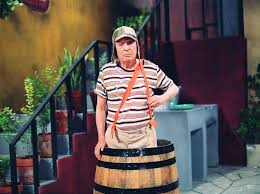
\includegraphics[width=5cm,height=2cm,keepaspectratio,trim=0 0 0 -5]{images/chaves/1.jpeg}
  \end{subfigure}
   & 
    \begin{subfigure}[b]{5cm}
  \centering
   
\includegraphics[width=5cm,height=2cm,keepaspectratio,trim=0 0 0 -5]{images/chaves/2.jpeg}
  \end{subfigure} \\ 
 \hline
   \begin{subfigure}[b]{5cm}
  \centering
   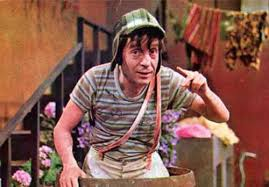
\includegraphics[width=5cm,height=2cm,keepaspectratio,trim=0 0 0 -5]{images/chaves/3.jpeg}
   
  \end{subfigure}
   &
   \begin{subfigure}[b]{5cm}
  \centering
   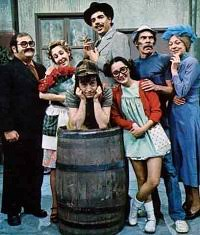
\includegraphics[width=5cm,height=2cm,keepaspectratio,trim=0 0 0 -5]{images/chaves/4.jpeg}
	
   \end{subfigure}
   & 
   \begin{subfigure}[b]{5cm}
  \centering
    
\includegraphics[width=5cm,height=2cm,keepaspectratio,trim=0 0 0 -5]{images/chaves/5.jpeg}
    
  \end{subfigure} \\ 
   \hline
   \begin{subfigure}[b]{5cm}
  \centering
   
\includegraphics[width=5cm,height=2cm,keepaspectratio,trim=0 0 0 -5]{images/chaves/6.jpeg}
   
  \end{subfigure}
   &
   \begin{subfigure}[b]{5cm}
  \centering
   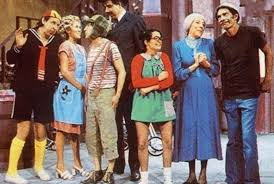
\includegraphics[width=5cm,height=2cm,keepaspectratio,trim=0 0 0 -5]{images/chaves/7.jpeg}
	
   \end{subfigure}
   & 
   \begin{subfigure}[b]{5cm}
  \centering
    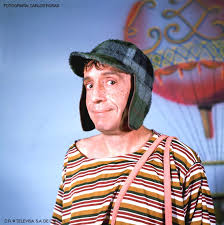
\includegraphics[width=5cm,height=2cm,keepaspectratio,trim=0 0 0 -5]{images/chaves/8.jpeg}
    
  \end{subfigure} \\ 
   \hline
   \begin{subfigure}[b]{5cm}
  \centering
   
\includegraphics[width=5cm,height=2cm,keepaspectratio,trim=0 0 0 -5]{images/chaves/9.jpeg}
   
  \end{subfigure}
   &
   \begin{subfigure}[b]{5cm}
  \centering
   
\includegraphics[width=5cm,height=2cm,keepaspectratio,trim=0 0 0 -5]{images/chaves/10.jpeg}
	
   \end{subfigure}
   & 
   \begin{subfigure}[b]{5cm}
  \centering
    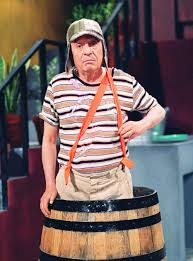
\includegraphics[width=5cm,height=2cm,keepaspectratio,trim=0 0 0 -5]{images/chaves/11.jpeg}
    
  \end{subfigure} \\ 
   \hline
   \begin{subfigure}[b]{5cm}
  \centering
   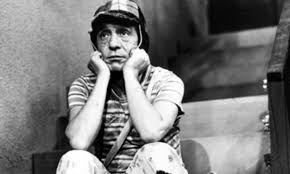
\includegraphics[width=5cm,height=2cm,keepaspectratio,trim=0 0 0 -5]{images/chaves/12.jpeg}
   
  \end{subfigure}
   &
   \begin{subfigure}[b]{5cm}
  \centering
   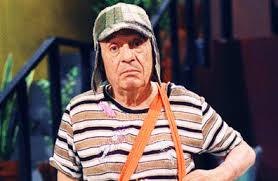
\includegraphics[width=5cm,height=2cm,keepaspectratio,trim=0 0 0 -5]{images/chaves/13.jpeg}
	
   \end{subfigure}
   & 
   \begin{subfigure}[b]{5cm}
  \centering
    
\includegraphics[width=5cm,height=2cm,keepaspectratio,trim=0 0 0 -5]{images/chaves/14.jpeg}
    
  \end{subfigure} \\ 
   \hline
   \begin{subfigure}[b]{5cm}
  \centering
   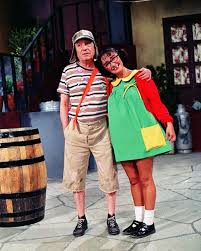
\includegraphics[width=5cm,height=2cm,keepaspectratio,trim=0 0 0 -5]{images/chaves/15.jpeg}
   
  \end{subfigure}
   &
   \begin{subfigure}[b]{5cm}
  \centering
   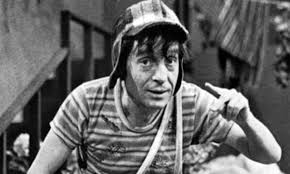
\includegraphics[width=5cm,height=2cm,keepaspectratio,trim=0 0 0 -5]{images/chaves/16.jpeg}
	
   \end{subfigure}
   & 
   \begin{subfigure}[b]{5cm}
  \centering
    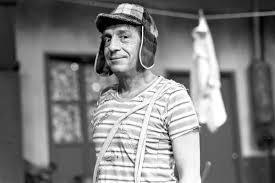
\includegraphics[width=5cm,height=2cm,keepaspectratio,trim=0 0 0 -5]{images/chaves/17.jpeg}
    
  \end{subfigure} \\ 
   \hline
   \begin{subfigure}[b]{5cm}
  \centering
   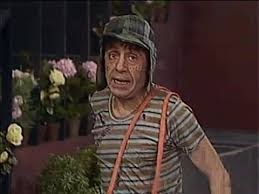
\includegraphics[width=5cm,height=2cm,keepaspectratio,trim=0 0 0 -5]{images/chaves/18.jpeg}
   
  \end{subfigure}
   &
   \begin{subfigure}[b]{5cm}
  \centering
   
\includegraphics[width=5cm,height=2cm,keepaspectratio,trim=0 0 0 -5]{images/chaves/19.jpeg}
	
   \end{subfigure}
   & 
   \begin{subfigure}[b]{5cm}
  \centering
    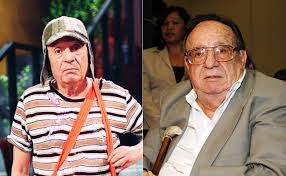
\includegraphics[width=5cm,height=2cm,keepaspectratio,trim=0 0 0 -5]{images/chaves/20.jpeg}
    
  \end{subfigure} \\ 
   \hline
   \begin{subfigure}[b]{5cm}
  \centering
   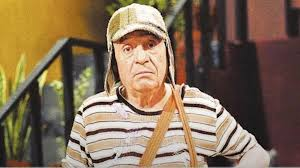
\includegraphics[width=5cm,height=2cm,keepaspectratio,trim=0 0 0 -5]{images/chaves/21.jpeg}
   
  \end{subfigure}
   &
   \begin{subfigure}[b]{5cm}
  \centering
   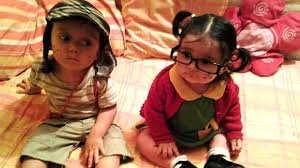
\includegraphics[width=5cm,height=2cm,keepaspectratio,trim=0 0 0 -5]{images/chaves/22.jpeg}
	
   \end{subfigure}
   & 
   \begin{subfigure}[b]{5cm}
  \centering
    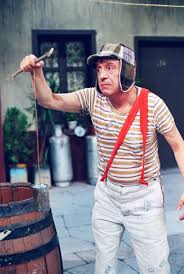
\includegraphics[width=5cm,height=2cm,keepaspectratio,trim=0 0 0 -5]{images/chaves/23.jpeg}
    
  \end{subfigure} \\
 \hline
 \begin{subfigure}[b]{5cm}
  \centering
   
\includegraphics[width=5cm,height=2cm,keepaspectratio,trim=0 0 0 -5]{images/chaves/24.jpeg}
   
  \end{subfigure}
   &
   \begin{subfigure}[b]{5cm}
  \centering
   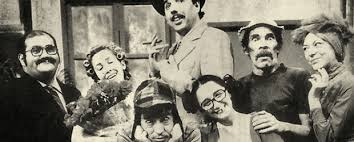
\includegraphics[width=5cm,height=2cm,keepaspectratio,trim=0 0 0 -5]{images/chaves/25.jpeg}
	
   \end{subfigure}
   & 
   \begin{subfigure}[b]{5cm}
  \centering
    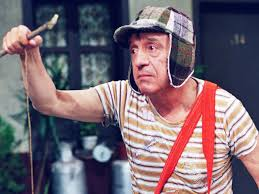
\includegraphics[width=5cm,height=2cm,keepaspectratio,trim=0 0 0 -5]{images/chaves/26.jpeg}
    
  \end{subfigure} \\
 \hline\begin{subfigure}[b]{5cm}
  \centering
   
\includegraphics[width=5cm,height=2cm,keepaspectratio,trim=0 0 0 -5]{images/chaves/27.jpeg}
   
  \end{subfigure}
   &
   \begin{subfigure}[b]{5cm}
  \centering
   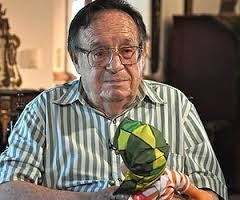
\includegraphics[width=5cm,height=2cm,keepaspectratio,trim=0 0 0 -5]{images/chaves/28.jpeg}
	
   \end{subfigure}
   & 
   \begin{subfigure}[b]{5cm}
  \centering
    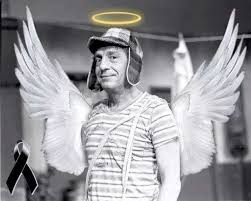
\includegraphics[width=5cm,height=2cm,keepaspectratio,trim=0 0 0 -5]{images/chaves/29.jpeg}
    
  \end{subfigure} \\
 \hline
 \begin{subfigure}[b]{5cm}
  \centering
   
\includegraphics[width=5cm,height=2cm,keepaspectratio,trim=0 0 0 -5]{images/chaves/30.jpeg}
   
  \end{subfigure}
   &
   &  \\
 \hline
\end{tabular}
\label{chaves}
\legend{\textbf{Fonte:} Autoria Própria.}
\end{center}
\end{table}